\documentclass[12pt, a4paper]{article}
\parindent0pt
\usepackage{fullpage}
\usepackage[utf8]{inputenc}
\usepackage[round]{natbib}
\usepackage{blindtext}
\usepackage{titlesec}
\usepackage{graphicx}
\bibliographystyle{plainnat}

\linespread{1.6}

\clubpenalty10000
\widowpenalty10000
\displaywidowpenalty=10000

\title{Were they able to know the danger? \\ The avalanche disaster from the 25th January 1689 in Saas im Prättigau.}
\author{Markus Graf}

\titleformat*{\section}{\normalfont\sffamily\bfseries}

\begin{document}
\maketitle
\abstract{\noindent The chronicles about the avalanche disaster from the 25th January 1689 don't reveal any reasons that 
led to this event. Only recent researches revealed that the lack of protection forest in combination with heavy snowfalls 
was the cause. There are no direct  sources that can answer whether they knew about the danger. But discussions about 
deforestation in that region and the knowledge about protection forest in other parts of Switzerland suggests that they were 
able to know consequences of deforestation and therefore to be aware of the danger. }

\newpage
\setlength{\parindent}{0pt}

\section*{The avalanche disaster from the 25th January 1689}
Daniel Jost a witness of the tragedy wrote in his chronicles\footnote{Translated from \citet[p.~50-51]{hansemann1995saaser}}:
\begin{quote}
\setlength{\parskip}{1.5em} 
``It was the day named  conversion of St. Paul, at the 25 of January 1689 at 8 o'clock, when we had to feel wrath of the 
highest of all God, as two dry avalanches went over the community of Saas, and in which 59 people lost their lives. 
From the community of Saas died 48, five from Conters, two from Fideris, three from Davos and one from Küblis.
 
The first avalanche, which went off at 8 o'clock, started outwards at Calmur in Büel, called the ``Hannen''; from that point 
on it rolled down the mountain through the forest down till Marthels and from there to the Landquartstutz. Cruelly it tore 
down forest, stables, houses and arboretums. The avalanche destroyed 10 houses, 15 people died and several were dug out alive.
An older woman for example was buried with the first avalanche and two girls with the second. They could not be dugged out until the next day.

After the first avalanche,  about 9 o'clock,  a good amount of friends  and neighbours were running for help because of the 
miserable screams and the raging church bells.The damage the avalanche caused was not visible from Conters because of the 
wind and weather. Also from Küblis side people were running for help. They dug out people and livestock till 12 o'clock. 
At this hour another avalanche went off. It started at Calandagrat and went down the mountain across Drumalinis, over 
the Barglein at Gruob, across the Landwasser. Finally the other side of the valley was covered with wood and household effects.
Also this avalanche tore down everything in front of it. It destroyed 12 houses, 44 people rest death or died later from the 
consequences. Most of the rescue team was beaten down while escaping. Only people escaped torwards the center of the village  got away. Several begun to work again, others fled. At this hour a group of people from Serneus went to help. 
We dug out alive five persons from a pile on junior Rudolf Brosis house. We wish a cheerful resurrection to those who passed 
away to God, the Lord and a blessed end to the survivors. Many were dug out alive, many were healthy, several were injured, 
those I wish patience and get well. But those who lost all their belongings, those console oneself with Hiobs words of the 
first chapter in verse 21: And said, naked came I out of my mother's womb, and naked shall I return thither: the lord gave, 
and the lord had taken away; blessed be the name of the lord. They buried all corpses within nine weeks, most of them were 
intact as they died in their beds. 

After the second avalanche several people worked till midnight and dug out people death and alive at all times. 
They buried first 23 bodies in the churchyard of Saas, three in Conters and one in Küblis. The other time 12 in Saas, 
and the third time six. 

I, Daniel Jost from Conters, witnessed the events with my own eyes. I recognized the second avalanche and tried to warn 
them to escape inwards by shouting and whistling imploringly. Half of the people fled inwards where knocked but stayed 
alive, the others who fled outwards all died. I fled, was frightened and scared, I can not tell more of this event.''
\end{quote}

\setlength{\parskip}{1.5em}

More then 300 years later, nothing reminds on the tragedy Daniel Jost witnessed in this winter. The area where the avalanches 
went down is now cluttered with new houses. A good portion of them are secondary homes hosting tourists. Weather forecasts, 
risk assessments, forestation, avalanche barrier and emergency plans makes it safe to live there. Because of a strong winter, 
an evacuation of the area Raschnal was necessary in 2009, but luckily nothing happened. Today people know about the dangers 
and authorities know how to deal with this threats. 

The report form Jost is leaving behind a feeling of sorrow and raises the question whether they knew about the danger or 
was it coming out of the blue? One of the interesting fact is that none of the reports questioned the reason or the 
circumstances of that event. Jost was just speaking of the wrath of God. None of the reports that is available in the Saaser 
hometown book\footnote{\citet[p.~50-54]{hansemann1995saaser}} is discussing the cause of this event. 

\section*{Learning from the past -  Reconstruction of the event from 1689 reveals the reason behind the tragedy}
A hazard assessment including a map of risk was done for Saas im Prättigau in 2004\footnote{\cite{teufen2004}}. 
They analysed  the event in January 1689 to answer the question whether such a disaster is still possible today.  
Based on the report from the chronicles of Jost, estimation off the type, the dimensions and the track of the avalanches was 
made. It was concluded that an avalanche with the same properties would not reach the same force again today. 
The difference between now and then was the the forestation along the track of the avalanche. The absence of protection 
forest was the only conceivable reason how the avalanche built such a massive force. 

The theory about the lack of forest is also supported by a myth around this event, in which a child-cradle was blown over 
the river to the other side of the valley whereas the child stayed uninjured\footnote{\citet[p.~53]{hansemann1995saaser}}. 
The track of the avalanche was described as following: ``The mountain slope above the village takes about two hour steep 
upwards and consists of beautiful meadows interrupted by small strips of forest.''

Not only the topographical properties were decisive factors, to build such an intense avalanche, it also needs a good amount 
of snow that triggers the drift. The weather conditions were also reported in the 
myth\footnote{\citet[p.~53]{hansemann1995saaser}}. It was snowing for two weeks before the event. On the same day, another 
avalanche went off in St.Antönien, a community nearby. The event was written down in the Ruosch chronicles and it confirms 
that snowfalls were immense in this region, so that Finze-Michaelsen describes it as catastrophic Winter\footnote{\citet[p.~18]{finze1988geschichte}}.  

\begin{figure}
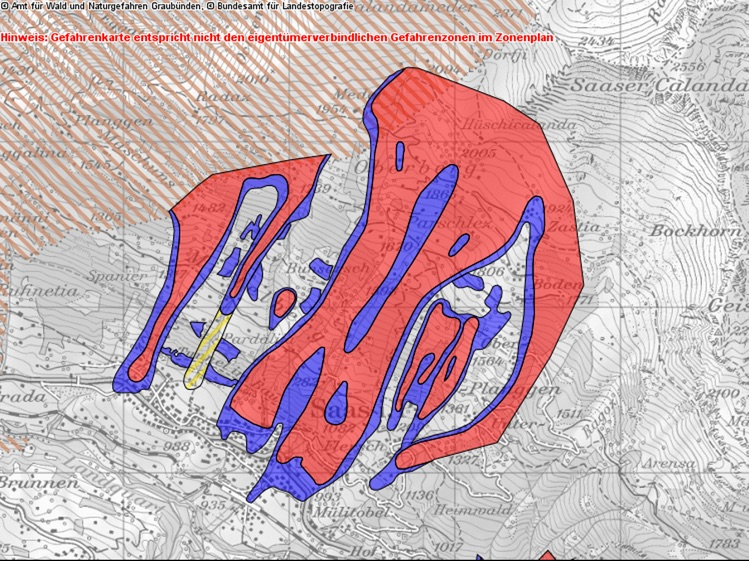
\includegraphics[width=\textwidth,natwidth=610,natheight=642]{literature/gefahrenkarte.jpg}
\caption{Map of risk for Saas im Prättigau \citep{gefahrenkarte}}
\end{figure}

\section*{The history of protection forest in Switzerland}
People are save today especially because of forestation that protects people below the slope. To discuss wether people from 
Saas im Prättigau knew the danger we first have to review the history of protection forest in Switzerland.

Today a protection forest is by definition an area covered by forest to protect against avalanches, rockfall, mudflow, 
or flooding. The term varies in its meaning, especially the German term ``Bannwald''. The historical meaning of ``Bann'' 
is an area that is controlled by a landlord where nobody is allowed to use it without his permission. In medieval times 
the Bannwald was a protected forest and only in  modern times the word is used as forest that protects people from natural 
disasters.

One of the first known Swiss letter that prohibits the use of the forest to protect people was found in Andermatt 
from 1397\footnote{\citet[p.~104]{pfister2002tag}}. Every use of wood, also deadwood was prohibited. People knew that 
the forest prevents avalanches from going off. Protected forests were sometimes also guarded by local forest and field 
warden, but the reason behind this was mostly just to protect the property and not to maintain the protective function. 

But simple people had no other chance as clearing the forest in higher areas. They needed the wood for constructing and 
heating, therefore they simply had no alternatives. So the forest was thinned out anyway, especially in the 17th century. 
Only in the 19th century people started to question this actions, especially because a huge amount of floods happend. 
Until then forest protection concerned only the cantons. Strong political pressure led 1874 to a new section in the federal 
constitution that authorizes federal government to manage Swiss forest centrally. In 1876 all mountain side forests were 
protected and reforestation was subsidised. Every forest in Switzerland was protected by the forest police  
act 26 years later\footnote{\citet[p.~108]{pfister2002tag}}.

\section*{Discussion about the knowledge of protection forest in Saas im Prättigau}
The history of protection forest in Switzerland reveals that there were regions where people knew about the importance of 
forest to protect them from harm. There are other hints that people knew about the issue of deforestation in this region. 

The parish letter of Saas im Prättigau around 1550 reveals, that there were already strict rules concerning the cutting of 
timber. Hansenmann is speculating that one reason for this regulation was the smelting works that needed a lot of wood. 
He also states that a lot of challenges the community is still facing today were already present in the past, especially 
avalanches and mudflows\footnote{\citet[p.~27, 139]{hansemann1995saaser}}.

Regarding the sustainability of the forest another interesting quote can be found in \citet[p.~7]{finze1988geschichte}, 
in which chronicler Georg Engle 1807 is writing that people from St.Antönien are already complaining 300 years ago about 
deforestation and waste of wood that is no longer available for their offspring. 

Putting everything together, there is no explicit source that describes that people of Saas im Prättigau knew about the 
danger, especially in combination with this hard winter and the lack of forest. There is also no source that describes 
any actions right after the tragic event of 1689. But we certainly know that deforestation regarding the protection of 
ownership and sustainability was a known issue. We also know that knowledge off the consequences from deforestation 
regarding natural hazards was existing. From our perspective, such a transfer of knowledge was possible, especially because 
of the fact that Saas im Prättigau was and still is an important passage that connects Klosters and Davos with the 
Rhine Valley. It is possible that documents that governs actions after the avalanche regarding protection of the 
forest existed but got lost. One explanation could be the devastating fire of 1735 that destroyed the village especially the 
center with its church and probably ruined the archive containing government documents and other historical 
sources\footnote{\citet[p.~55]{hansemann1995saaser}}.

\begin{figure}
\begin{center}
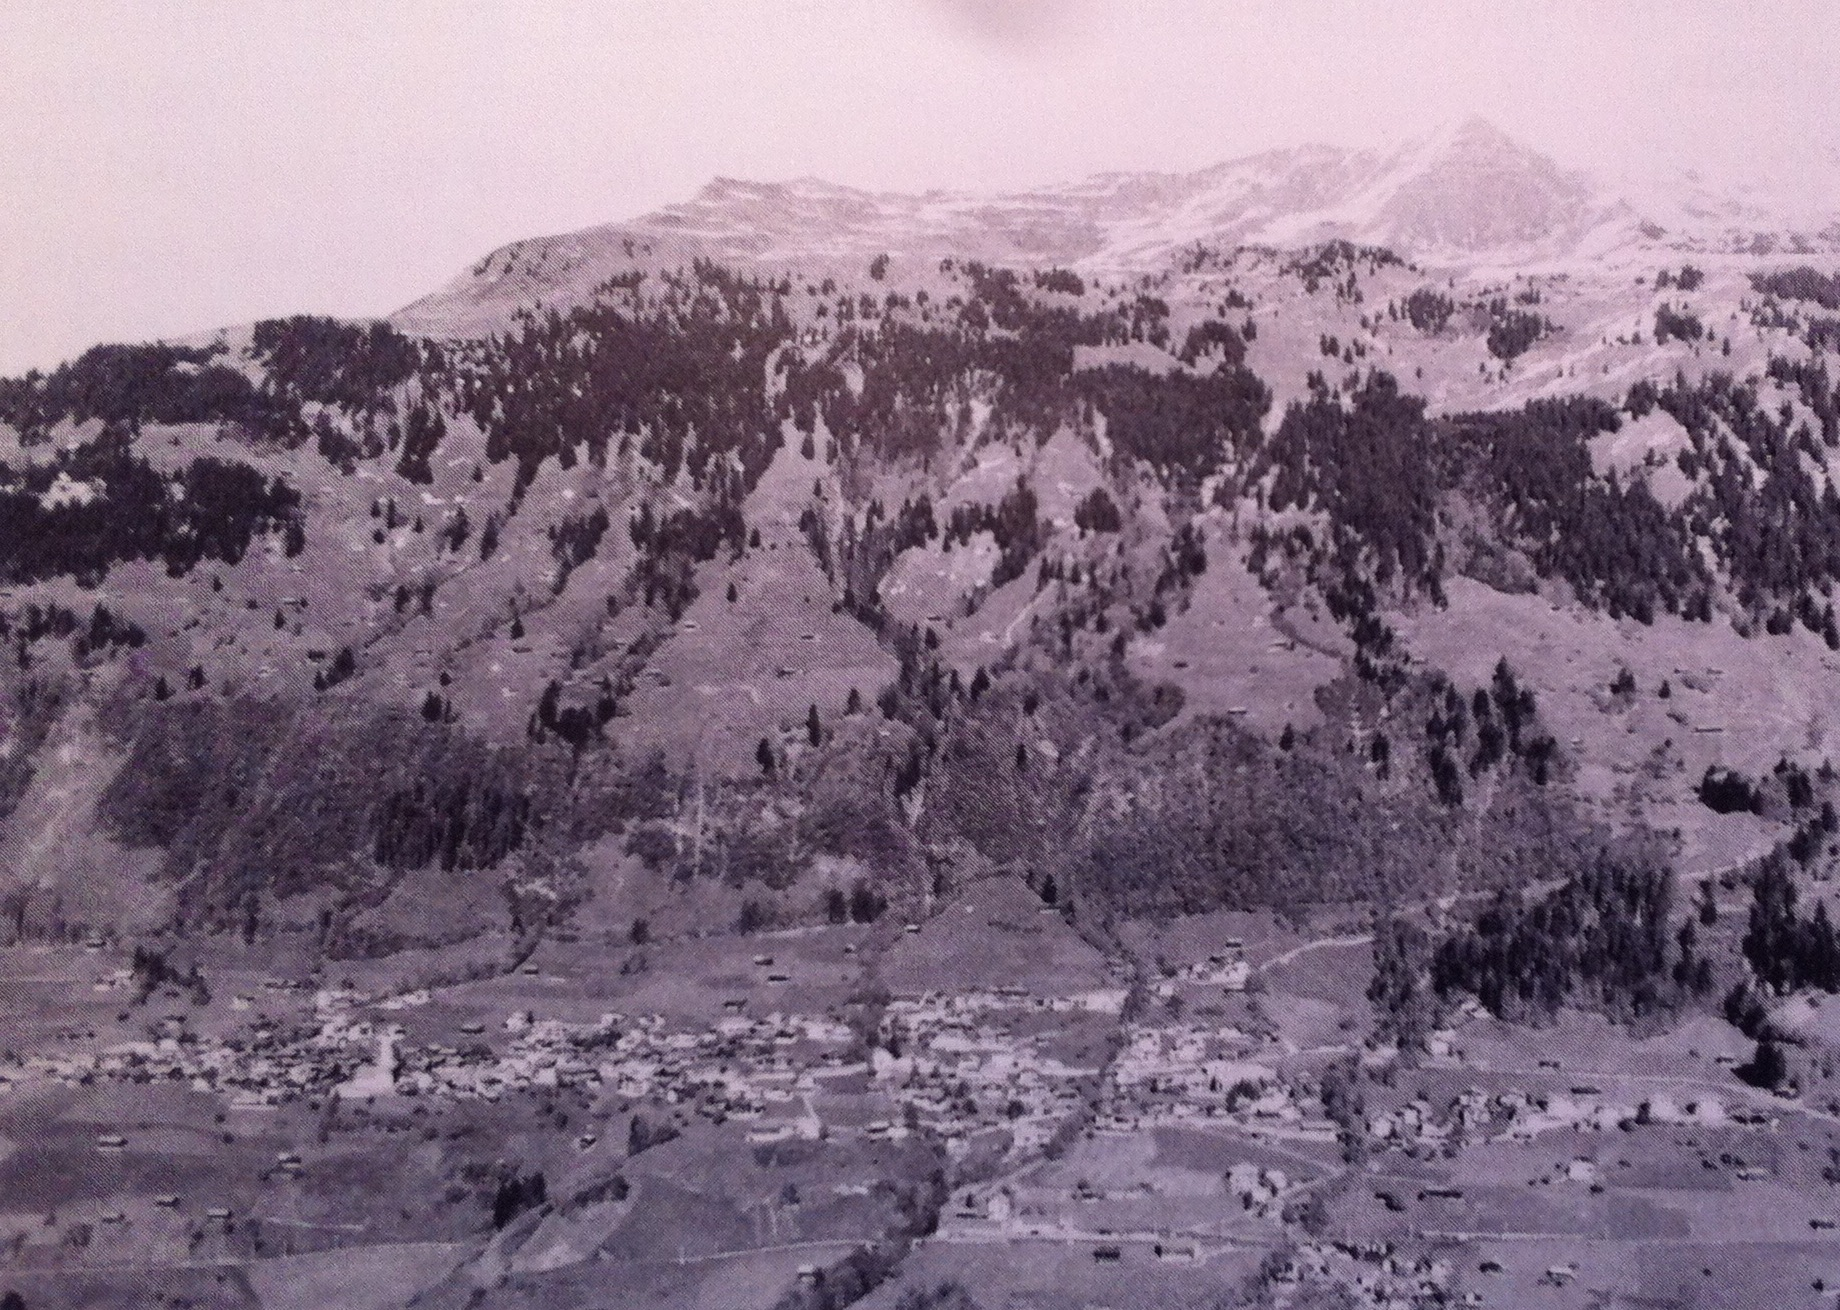
\includegraphics[width=\textwidth,natwidth=610,natheight=642]{literature/saas.jpg}
\end{center}
\caption{Saas im Prättigau, view from above Conter \citep[p.~216]{hansemann1995saaser}}
\end{figure} 


\section*{Perspectives of the future}
The importence of protection against natural hazards was gaining importance with better life quality and progresses of 
civilization and technology. It's unlikely that knowledge about the importance of the protection against avalanches in this 
region will be lost. But we learned that knowledge and memories of such a tragic event can fade away. It is important to 
conserve such events and keep in mind that such dangers existed and can reappear.

\bibliography{literature}
\end{document}
